\documentclass[tikz,border=2pt]{standalone}
\usepackage{xcolor}
\begin{document}
% IV*_-1
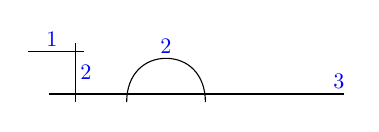
\begin{tikzpicture}[xscale=1,yscale=0.9]
\draw[thick,shorten >=2] (4/15,0)--(49/12,0) node[inner sep=2pt,blue,above left,scale=0.8] {3} node[inner sep=2pt,below left,scale=0.8] {};
\draw[shorten <=-3pt, shorten >=-3pt] (3/5,0)--node[inner sep=2pt,scale=0.8,blue,right] {2} (3/5,3/5);
\draw[shorten <=-3pt] (3/5,3/5)--node[inner sep=2pt,scale=0.8,blue,above] {1} (0,3/5);
\draw[shorten <=-3pt, shorten >=-3pt] (5/4,0) ++(1,0) arc (0:180:0.5) node[inner sep=2pt,scale=0.8,blue,midway,above] {2};
\end{tikzpicture}
\end{document}
